\section{Metodologia}
\subsection{Técnicas de pesquisa}

\begin{frame}{Metodologia e técnicas de pesquisa}
    \begin{block}{Mapeamento Sistemático (MS)}
    Identificar e classificar o conteúdo relacionado à \textbf{verificação para correção} ou \textbf{detecção de vulnerabilidades} para aprimoramento da segurança dos CIs.
    \end{block}
    Com base no MS:
    \begin{itemize}
        \item Seleção do método de verificação e detecção de vulnerabilidades;
        \item Seleção das vulnerabilidades abordadas;
        \item Definição da estratégia para validação da proposta. 
    \end{itemize}
\end{frame}

\subsection{Mapeamento Sistemático}
\begin{frame}{Mapeamento Sistemático}
    Três fases:
    \begin{itemize}
        \item Planejamento;
        \begin{itemize}
            \item Objetivo e protocolo do MS.
        \end{itemize}
        \item Condução;
        \begin{itemize}
            \item Identificação dos estudos primários;
            \item Extração e síntese dos dados.
        \end{itemize}
        \item Publicação dos resultados.
        \begin{itemize}
            \item Questões de pesquisa são respondidas;
            \item Relato dos resultados.
        \end{itemize}
    \end{itemize}
\end{frame}

\begin{frame}{Protocolo do MS}
\textbf{Questões de pesquisa}:
    \begin{itemize}
        \item \textbf{QP 1.} Quais abordagens têm sido propostas?
        \item \textbf{QP 2.} Quando e onde os estudos têm sido publicados?
        \item \textbf{QP 3.} Quais problemas ou vulnerabilidades relacionados aos CIs têm sido abordados?
        \item \textbf{QP 4.} Quais estratégias de validação foram utilizadas?
        \item \textbf{QP 5.} Quais são as limitações presentes nas abordagens?
    \end{itemize}    
\end{frame}

\begin{frame}{Protocolo do MS}
\textbf{String de busca}:
    \begin{center}
    (\textit{``smart contract'' OR ``ethereum bytecode''}) \textit{AND} (\textit{verification OR validation OR monitor* OR analysis OR formalization OR ``formal methods'' OR ``security vulnerabilities'' OR ``security bugs'' OR ``vulnerability detection'' OR ``bug detection'' OR optimiz*})
    \end{center}
\textbf{Motores de busca e bases bibliográficas}:
    \begin{itemize}
        \item \textit{Engineering Village};
        \item \textit{Scopus};
        \item \textit{Web of Science};
        \item \textit{IEEE Xplore};
        \item \textit{ACM Digital Library}.
    \end{itemize}
\end{frame}

\begin{frame}{Planejamento e condução}
    \begin{figure}[!htb]
     \centering
     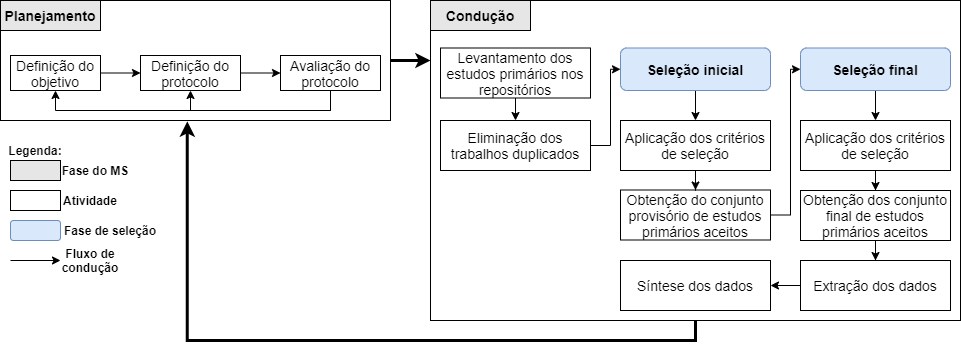
\includegraphics[scale=0.3]{figuras/metodologia/ms_fluxo.png}
    \end{figure}
    \begin{itemize}
        \item Total de estudos selecionados: 2091
        \item Total de estudos aceitos: \textbf{104}
    \end{itemize}
\end{frame}

\begin{frame}{Resultados - QP1}
    \begin{itemize}
        \item \textbf{QP1.} Quais abordagens têm sido propostas?
    \end{itemize}
    \begin{figure}[!htb]
     \centering
     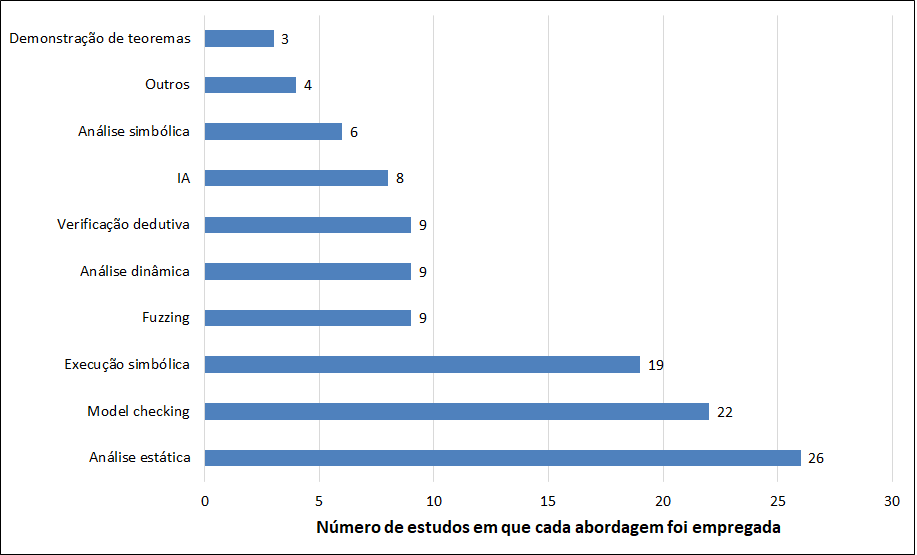
\includegraphics[scale=0.4]{figuras/metodologia/rq1-abordagens.png}
    \end{figure}
\end{frame}

\begin{frame}{Resultados - QP2}
    \begin{itemize}
        \item \textbf{QP2.} Quando e onde os estudos têm sido publicados?
    \end{itemize}
    \begin{figure}[!htb]
     \centering
     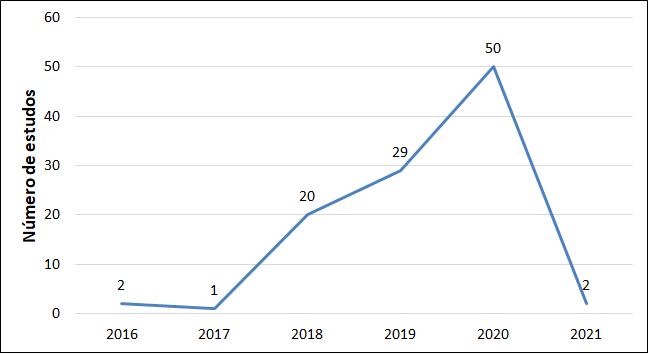
\includegraphics[scale=0.5]{figuras/metodologia/rq2-distribuicao-estudos.png}
    \end{figure}
\end{frame}

\begin{frame}{Resultados - QP2}
    \begin{itemize}
        \item \textbf{QP2.} Quando e onde os estudos têm sido publicados?
    \end{itemize}
    \begin{figure}[!htb]
     \centering
     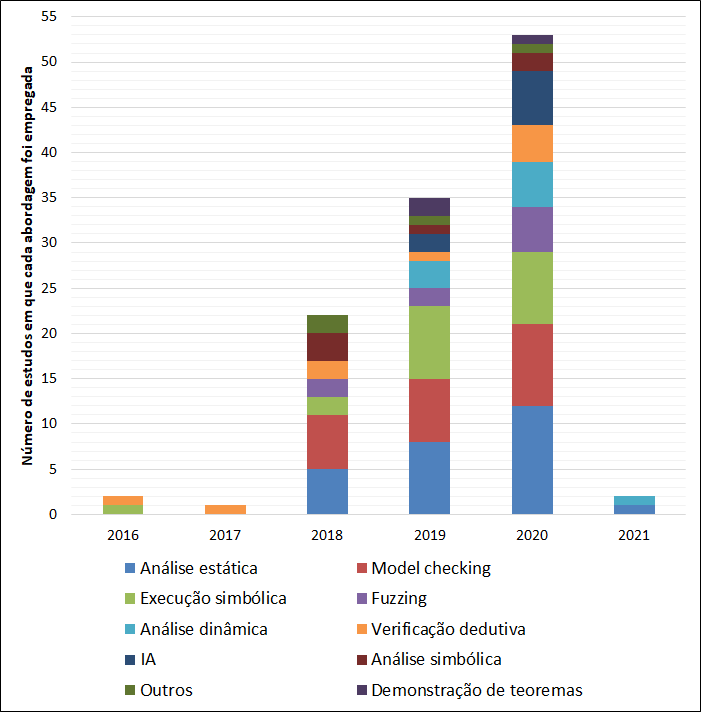
\includegraphics[scale=0.35]{figuras/metodologia/rq2-distribuicao-abordagens.png}
    \end{figure}
\end{frame}

\begin{frame}{Resultados - QP3}
    \begin{itemize}
        \item \textbf{QP3.} Quais problemas ou vulnerabilidades relacionados aos CIs têm sido abordados?
    \end{itemize}
    \begin{figure}[!htb]
     \centering
     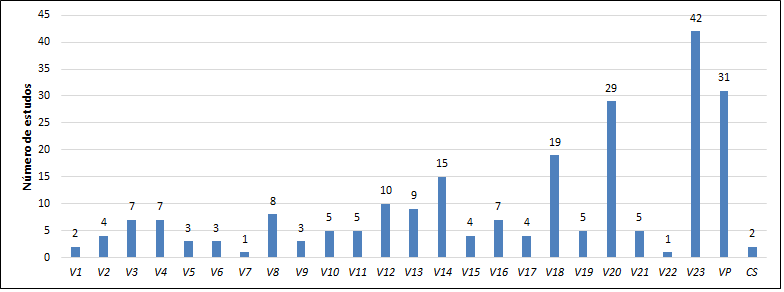
\includegraphics[scale=0.55]{figuras/metodologia/rq3-vulnerabilidades.png}
    \end{figure}    
\end{frame}

\begin{frame}{Resultados - QP3}
    \begin{itemize}
        \item \textbf{QP3.} Quais problemas ou vulnerabilidades relacionados aos CIs têm sido abordados?
    \end{itemize}
    \begin{table}[!ht]
\centering
\fontsize{8pt}{8pt}\selectfont
\caption{Vulnerabilidades e problemas alvos de verificação em CIs}
\label{tab:rq3-vulnerabilidades}
\begin{tabular}{@{}llll@{}}
\toprule
\textbf{Sigla} & \textbf{Vulnerabilidade / Problema} & \textbf{Sigla} & \textbf{Vulnerabilidade / Problema} \\ \midrule
$V_{1}$  & Ataque de profundidade da pilha de chamadas & $V_{14}$ & Dependência de \textit{timestamp}       \\
$V_{2}$  & Ataque DoS com operações ilimitadas         & $V_{15}$ & Desordem de exceções           \\
$V_{3}$  & Autenticação com \textit{tx.origin}                  & $V_{16}$ & Divisão por zero               \\
$V_{4}$  & Bloqueio de Ether                           & $V_{17}$ & Endereço curto                 \\
$V_{5}$  & Consumo de \textit{gas} ineficiente                  & $V_{18}$ & Exceções não tratadas          \\
$V_{6}$  & Contrato guloso                             & $V_{19}$ & Chamada externa não verificada \\
$V_{7}$  & Contrato pródigo                            & $V_{20}$ & \textit{Integer overflow} e \textit{underflow}   \\
$V_{8}$  & Contrato suicida                            & $V_{21}$ & Gasto de \textit{gas} descontrolado     \\
$V_{9}$  & Contrato \textit{honeypot}                           & $V_{22}$ & Problemas de concorrência      \\
$V_{10}$ & Controle de acesso vulnerável               & $V_{23}$ & Reentrância                    \\
$V_{11}$ & \textit{Delegatecall injection}             & $VP$  & Violação de propriedades       \\
$V_{12}$ & Dependência de informação do bloco          & $CSS$ & Correção sintática e semântica \\
$V_{13}$ & Dependência de ordem da transação           &       &                                \\ \bottomrule
\end{tabular}
\end{table}
\end{frame}

\begin{frame}{Resultados - QP4}
    \begin{itemize}
        \item \textbf{QP4.} Quais estratégias de validação foram utilizadas?
    \end{itemize}
    \begin{figure}[!htb]
     \centering
     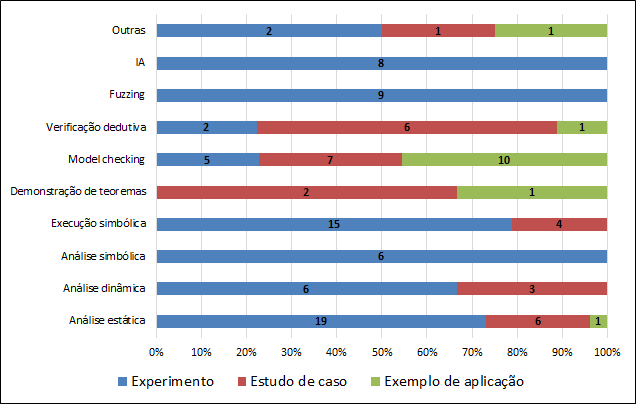
\includegraphics[scale=0.5]{figuras/metodologia/rq4-validacao-propostas.png}
    \end{figure}    
\end{frame}

\begin{frame}{Resultados - QP5}
    \begin{itemize}
        \item \textbf{QP5.} Quais são as limitações presentes nas abordagens?
    \end{itemize}
    \begin{figure}[!htb]
     \centering
     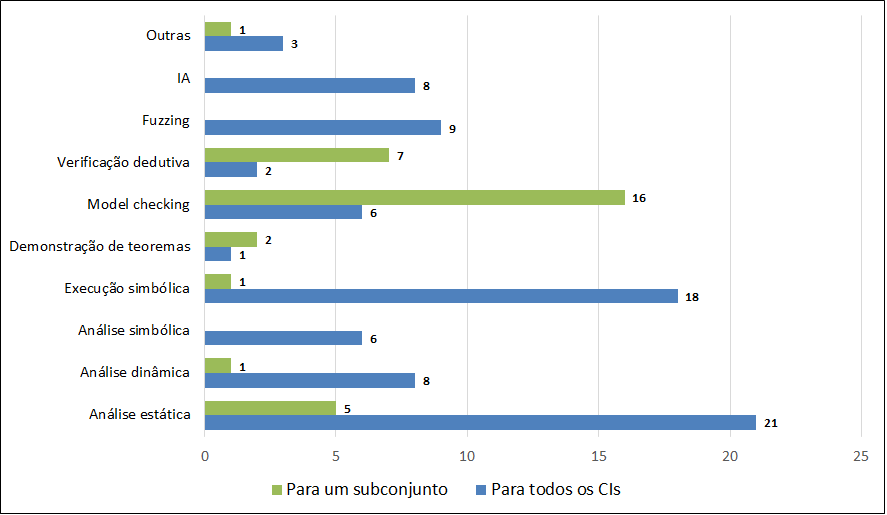
\includegraphics[scale=0.4]{figuras/metodologia/rq5-abrangencia.png}
    \end{figure}     
\end{frame}

\begin{frame}{Resultados - QP5}
    \begin{itemize}
        \item \textbf{QP5.} Quais são as limitações presentes nas abordagens?
    \end{itemize}
    \begin{figure}[!htb]
     \centering
     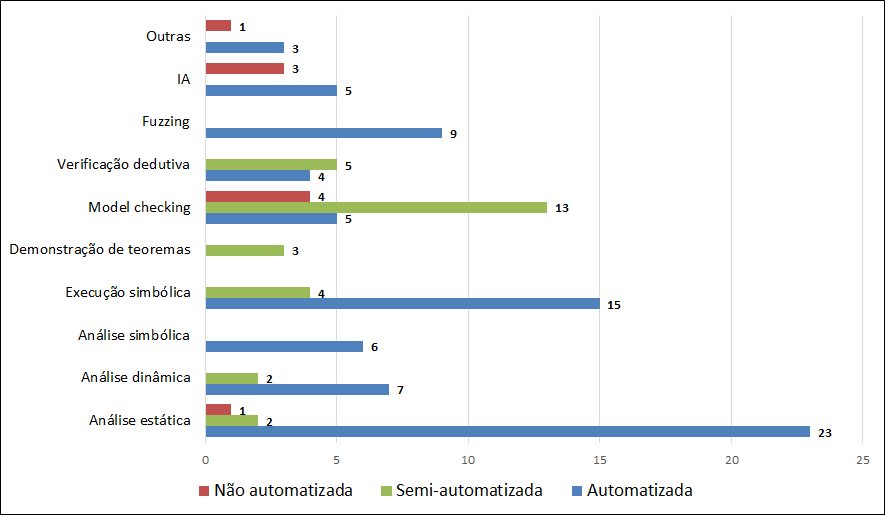
\includegraphics[scale=0.4]{figuras/metodologia/rq5-automacao.png}
    \end{figure}     
\end{frame}

\begin{frame}{Discussão}
    \begin{itemize}
        \item \textit{Model checking} está entre as abordagens mais utilizadas nos últimos anos;
        \item Há poucos estudos com validação experimental;
        \item Reentrância foi a vulnerabilidade mais abordada;
        \item A violação de propriedades 
    \end{itemize}
\end{frame}

%abrangência
%nível de automação
%conhecimento prévio
%acurácia - FP ou FN